\documentclass[letterpaper,12pt]{article}
\usepackage[spanish]{babel}
\spanishdecimal{.}
\selectlanguage{spanish}
\usepackage[spanish,onelanguage,ruled]{algorithm2e}
\usepackage[utf8]{inputenc}
\usepackage{graphicx}
\usepackage{caption}
\usepackage{subcaption}
\usepackage[top=2cm, bottom=2cm, left=2cm, right=2cm]{geometry}
\usepackage{hyperref}
\usepackage{verbatim}
\usepackage{amssymb}
\usepackage{mathtools}
\newcommand\ddfrac[2]{\frac{\displaystyle #1}{\displaystyle #2}}

\title{Práctica 5  \\ Cálculo de rutas utilizando A* y celdas de ocupación}
\author{Laboratorio de Bio-Robótica}
\date{Robots Móviles y Agentes Inteligentes}
\begin{document}
\renewcommand{\tablename}{Tabla}
\maketitle
\section*{Objetivos}
\begin{itemize}
\item A partir del mapa creado en la práctica 4, calcular una ruta mediante el algoritmo A*.
\item Suavizar la ruta utilizando descenso del gradiente. 
\item Publicar la ruta en un tópico y desplegarla en el visualizador \texttt{rviz}.
\end{itemize}

\section{Marco Teórico}
\subsection{El algoritmo A*}
La planeación de rutas consiste en la obtención de un movimiento continuo libre de colisiones que conecte una configuración inicial, con una final. Se asume que se dispone de una representación del ambiente con información sobre el espacio navegable y el ocupado por los obstáculos. En esta práctica se considera que el robot sólo se mueve sobre un plano y que se tiene una representación que consiste en un mapa de celdas de ocupación (obtenido en la práctica 4). 

Una posible solución es aplicar un algoritmo de búsqueda en grafos. En el caso de las celdas de ocupación, cada celda representa un nodo en el grafo y se considera que está conectada únicamente con aquellas celdas vecinas que pertenezcan al espacio libre. Para determinar los nodos vecinos se puede utilizar conectividad cuatro u ocho. En esta práctica se utilizará la conectivad cuatro. 

A* es un algoritmo de búsqueda que explora la ruta con el menor costo esperado. Para un nodo $n$, el costo esperado $f(n)$ se calcula como 
\[f(n) = g(n) + h(n)\]
donde $g(n)$ es el costo de la ruta desde el nodo origen hasta el nodo $n$ y $h(n)$ es una heurística que determina \textit{un} costo que se esperaría tener desde el mismo nodo $n$ hasta el nodo objetivo. Este costo esperado de hecho subestima el valor real, es decir, se debe cumplir que $h(n) \leq g(n)\quad \forall\; n \in\; Grafo$. 

En la búsqueda por A* se manejan dos conjuntos principales: la \textit{lista abierta} y la \textit{lista cerrada}. La lista abierta contiene todos los nodos que han sido visitados pero no expandidos y la cerrada, aquellos que han sido visitados \textit{y} expandidos (también llamados nodos conocidos). El algoritmo \ref{alg:AStar} muestra los pasos en pseudocódigo para implementar A*. 
\begin{algorithm}
\DontPrintSemicolon
\KwData{Grafo, nodo inicial, nodo meta}
\KwResult{Ruta óptima expresada como una secuencia de nodos}
Cerrado $\leftarrow \emptyset$\;
Abierto $\leftarrow$ \{nodo\_inicial\}\;
previo(nodo\_inicial) $\leftarrow \varnothing$\;
\While{ Abierto $\neq\emptyset$ }
{
  nodo\_actual $\leftarrow$ nodo con el menor valor $f$ del conjunto $Abierto$\;
  Abierto $\leftarrow$ Abierto - \{nodo\_actual\}\;
  Cerrado $\leftarrow$ Cerrado $\cup$ \{nodo\_actual\}\;
  \If{nodo\_actual es nodo\_meta}
  {
    Anunciar éxito y salir de este ciclo\;
  }
  \ForEach{nodo\_vecino de nodo\_actual}
  {
    \If{nodo\_vecino $\in$ Cerrado}{Continuar con el siguiente nodo\_vecino}
    \eIf{nodo\_vecino $\in$ Abierto}
    {
      costo\_temporal $\leftarrow g(\textrm{nodo\_actual}) + d(\textrm{nodo\_actual, nodo\_vecino})$\;
      \If{costo\_temporal $<$ g(nodo\_vecino)}
      {
        $g(\textrm{nodo\_vecino})\leftarrow$ costo\_temporal\;
        $f(\textrm{nodo\_vecino})\leftarrow$ costo\_temporal + heurística(nodo\_vecino, nodo\_meta)\;
        previo(nodo\_vecino) $\leftarrow$ nodo\_actual\;
      }
    }
    {
      $g(\textrm{nodo\_vecino})\leftarrow g(\textrm{nodo\_actual}) + d(\textrm{nodo\_actual, nodo\_vecino})$\;
      $f(\textrm{nodo\_vecino})\leftarrow g\textrm{nodo\_vecino})$  + heurística(nodo\_vecino, nodo\_meta)\;
      previo(nodo\_vecino) $\leftarrow$ nodo\_actual\;
      Abierto $\leftarrow$ Abierto $\cup$ \{nodo\_vecino\}\; 
    }
  }
}
\eIf{nodo\_actual $\neq$ nodo\_meta}
{
  Anunciar falla\;
}
{
  RutaOptima $\leftarrow\emptyset$ \;
  \While{nodo\_actual $\neq\varnothing$ }
  {
    \textit{//El nodo actual se inserta al principio de la ruta}\;
    RutaÓptima $\leftarrow$ \{nodo\_actual\} $\cup$ RutaÓptima \;
    nodo\_actual $\leftarrow$ previo(nodo\_actual)\;
  }
  Regresar RutaÓptima
}
\caption{Búsqueda con A*}
\label{alg:AStar}
\end{algorithm}

\subsection{Crecimiento de obstáculos}
Como se mencionó anteriormente, se asume que se tiene un mapa con información sobre el espacio libre y ocupado, sin embargo, en una implementación en un robot real, las celdas que están junto al espacio ocupado no se pueden considerar como libres ya que si el robot se mueve hacia ellas seguramente chocará con algo. Una forma de solucionar esto sería hacer las celdas tan grandes de modo que puedan contener al robot, sin embargo, esta resolución sería muy baja y la representación del ambiente sería muy mala. Otra posible solución es \textit{crecer} los obstáculos de modo que las celdas que están muy cerca del espacio ocupado se consideren también como ocupadas.

\begin{figure}
\centering
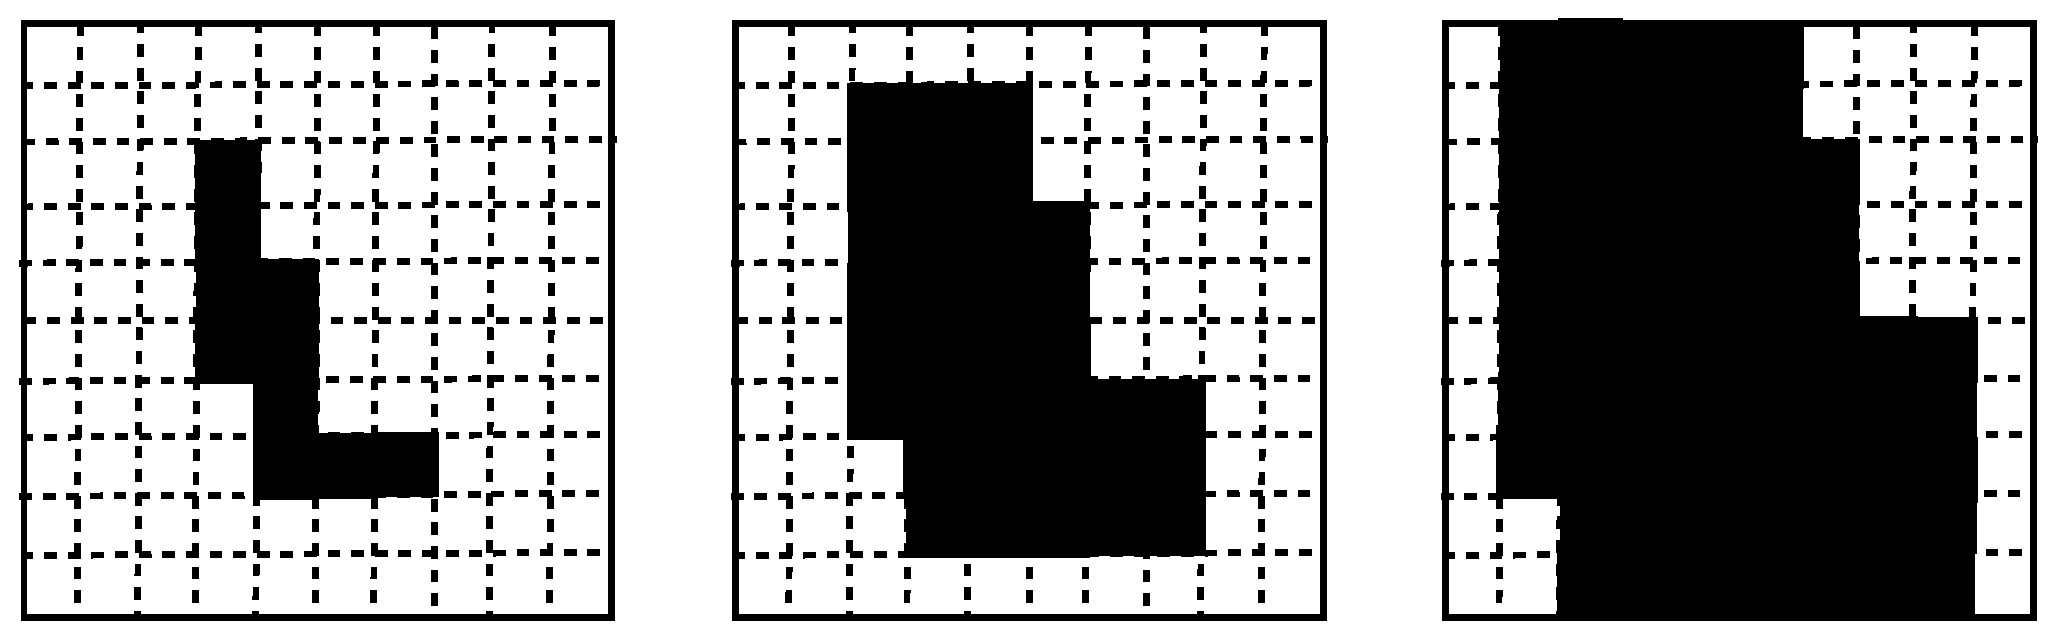
\includegraphics[width=0.8\textwidth]{Figures/Grow.eps}
\caption{Crecimiento de obstáculos}
\label{fig:Grow}
\end{figure}

La figura \ref{fig:Grow} muestra un ejemplo en el que los obstáculos se han aumentado dos celdas. Este procedimiento se conoce como \textit{dilatación} y es un tipo de \textit{operador morfológico}. La explicación de estos conceptos se hará en temas posteriores.

Los obstáculos deben aumentarse cuando menos el radio del robot. Para el mapa obtenido en la práctica 4, dado que la resolución es de 5[cm] y los robots utilizados tienen casi 0.5[m] de diámetro, los obstáculos deben aumentarse cuando menos 5 celdas. El algoritmo \ref{alg:Grow} enumera los pasos para crecer obstáculos en un mapa.

\begin{algorithm}
\DontPrintSemicolon
\KwData{Mapa de celdas de ocupación $M = \{c_0 ... c_n\}$, número de celdas a aumentar $k$.}
\KwResult{Mapa con los obstáculos aumentados.}
Repetir $k$ veces los siguientes pasos:\;
\ForAll{$c \in M$}
{
  \If{$c$ está en el espacio ocupado}
  {
    $V(c) \leftarrow $ Conjunto de celdas vecinas de $c$ (conectividad ocho)\;
    \ForAll{$v \in V(c)$}
    {
      Marcar $v$ como parte del espacio ocupado\;
    }
  }
}
Regresar $M$
\caption{Crecimiento de obstáculos.}
\label{alg:Grow}
\end{algorithm}


\subsection{Suavizado de la ruta: función de costo}
Dado que se está utilizando conectividad cuatro en el algoritmo de A*, la ruta calculada tendrá siempre vueltas con ángulos rectos, lo cual no es deseable por varias razones: la primera de ellas es que la función de posición no es diferenciable en las esquinas, además, este tipo de vueltas ocasionan cambios bruscos en las señales de control, lo que finalmente ocasiona daños a los motores de la base móvil. Por otro lado, las restricciones de movimiento en algunos tipos de bases (como es el caso de los automóviles) pueden impedir ejecutar vueltas en ángulo recto.

Por lo anterior, es conveniente suavizar la ruta calculada por A* de modo que la nueva ruta sea lo suficientemente parecida a la original pero al mismo tiempo, lo suficientemente suave para evitar curvas muy pronunciadas. La figura \ref{fig:Smooth} muestra un ejemplo de suavizado con dos casos extremos: la ruta roja es una ruta igual a la original, la azul es una ruta sin vueltas pero que ha dejado de ser una ruta útil, y la verde, que es un \textit{promedio ponderado} de las dos anteriores. 

Para poder obtener una ruta como la verde de la figura \ref{fig:Smooth}, plantearemos una función de costo que tome en cuenta el parecido con la ruta original y el \textit{nivel de suavizado} que se desee. Estos dos criterios están en conflicto: entre más suavizado, menor será el parecido con la ruta original y viceversa, es decir, la función de costo será grande con mucho suavizado y también debe ser muy grande si la ruta es muy parecida a la orignal. La idea es que dicha función de costo tenga un mínimo en un punto intermedio de modo que este punto corresponda a una ruta como la verde de la figura \ref{fig:Smooth}. 

Las funciones cuadráticas son una buena opción como función de costo ya que tienen un mínimo global y además son diferenciables. Para el suavizado de la ruta se propone la función de costo
\begin{equation}
V = \frac{1}{2}\alpha\sum_{i=1}^{n}\left(p_i - q_i\right)^2 + \frac{1}{2}\beta\sum_{i=1}^{n-1}\left(p_i - p_{i+1}\right)^2
\label{eq:Cost}
\end{equation}
donde $Q = \{q_1\dots q_n\}$ son todos los puntos $q = [x\,y]$ que forman la ruta original calculada con A* y $P=\{p_1\dots p_n\}$ son los puntos de la ruta ya suavizada. La constante $\alpha \geq 0$ es un parámetro de diseño para indicar cuánto peso se le quiere dar al parecido de la ruta original con la suavizada y $\beta \geq 0$ indica el peso que se le da al suavizado en sí. Con $\alpha = 0$ se obtendría una línea recta, como la ruta azul de la figura \ref{fig:Smooth}, y con $\beta = 0$ se obtendría una ruta igual a la original.

\begin{figure}
\centering
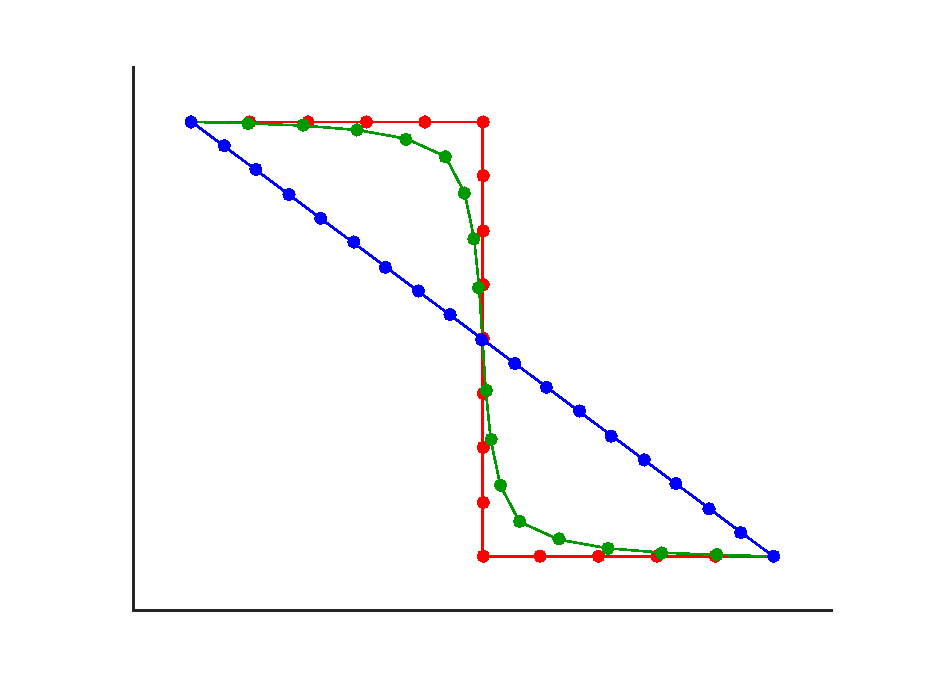
\includegraphics[width=0.5\textwidth]{Figures/Smooth.eps}
\caption{Ejemplos de suavizado}
\label{fig:Smooth}
\end{figure}

\subsection{Suavizado de la ruta: descenso del gradiente}
La ruta suavizada se obtiene encontrando el argumento que minimiza la función \ref{eq:Cost}, sin embargo, dada la cantidad tan grande de variables, es difícil encontrarlo analíticamente. Una forma más sencilla es mediante el médoto del descenso del gradiente, que consiste en mover el argumento pequeñas cantidades proporcionales al gradiente de la función $V$ y en sentido contrario a éste. Dado que el cambio entre cada iteración es proporcional a $\nabla V$, se puede asumir que cuando el cambio en el argumento es menor que una tolerancia, entonces se ha alcanzado el mínimo. 

El algoritmo \ref{alg:Gradient} contiene los pasos en pseudocódigo para implementar descenso del gradiente. La constante $\delta > 0$ debe ser lo suficientemente pequeña para evitar inestabilidad en el algoritmo, sin embargo, se debe considerar que entre más pequeña sea ésta, mayor será el costo computacional. 

\begin{algorithm}
\DontPrintSemicolon
\KwData{Función $V$ cuyo mínimo se desea encontrar, condición inicial $p(0)$, tolerancia $tol$.}
\KwResult{Argumento $p$ que minimiza $V$.}
$i = 0$\;
$p_i \leftarrow p(0)$\;
\While{ $\Vert\nabla V(p_i)\Vert > tol$}
{
\BlankLine
  $p_{i+1} \leftarrow p_i - \delta\nabla V(p_i)$\;
  $i \leftarrow i+1$
\BlankLine
}
Regresar $p_i$
\caption{Descenso del gradiente.}
\label{alg:Gradient}
\end{algorithm}

La ecuación \ref{eq:Cost} toma como argumentos las posiciones tanto de la ruta original como de la suavizada, sin embargo, dado que sólo varían los puntos de la nueva ruta, se puede considerar que el gradiente $\nabla V$ está dado por:
\begin{equation}
\underbrace{\left[\frac{}{}\alpha(p_1 - q_1)+\beta(p_1 - p_2)\right.}_{\ddfrac{\partial V}{\partial p_1}}
,\dots ,
\underbrace{\frac{}{}\alpha(p_i - q_i) + \beta(2p_i - p_{i-1} - p_{i+1})}_{\ddfrac{\partial V}{\partial p_i}}
,\dots ,
\underbrace{\left.\alpha(p_n-q_n)+\beta(p_n - p_{n-1})\frac{}{}\right]}_{\ddfrac{\partial V}{\partial p_n}}
\end{equation}
Nótese que se está derivando con respecto a $p$ (puntos de la ruta suavizada), no con respecto a $q$ (puntos de la ruta original). Recuerde que cada punto de la ruta tiene coordenadas $[x\,y]$, por lo que el descenso de gradiente se tiene que aplicar a ambas coordenadas. 

\section{Tareas}

\subsection{Prerrequisitos}
Antes de continuar, actualice el repositorio y recompile:
\begin{verbatim}
   cd ~/RoboticsCourses
   git pull origin master
   cd catkin_ws
   catkin_make
\end{verbatim}

Con el objetivo de facilitar las pruebas, se ha incluido un paquete llamado \texttt{navig\_msgs} que contiene un servicio llamado \texttt{CalculatePath}. El archivo se encuentra en \texttt{navig\_msgs/srv} y tiene el siguinte contenido:
\begin{verbatim}
   geometry_msgs/Pose start_pose
   geometry_msgs/Pose goal_pose
   nav_msgs/OccupancyGrid map
   ---
   nav_msgs/Path path
\end{verbatim}
La idea es utilizar este servicio en el nodo que calcula las rutas mediante A*. 

El paquete \texttt{map\_server} contiene un nodo del mismo nombre que publica periódicamente un mapa de celdas de ocupación y atiende un servicio con el que se puede obtener dicho mapa. Este nodo recibe por parámetro el nombre del archivo \texttt{.yaml} que contiene la información sobre el mapa a utilizar, en este caso, \texttt{biorobotics\_lab.yaml}. 

También se ha incluido una interfaz gráfica sencilla para facilitar el llamado del servicio \texttt{navig\_msgs/CalculatePath}. Esta interfaz se encuentra en en \texttt{catkin\_ws/src/hri/justina\_simple\_gui} y la figura \ref{fig:gui} muestra una captura de pantalla de ella. Cuando se presiona \texttt{enter} en alguno de los campos del cuadro \textit{Mobile base and navigation}, este programa llama al servicio de nombre \texttt{/navigation/a\_star} de tipo \texttt{navig\_msgs/CalculatePath} con los datos correspondientes en la parte de la petición (\texttt{start\_pose, goal\_pose} y \texttt{map}).
\begin{figure}
\centering
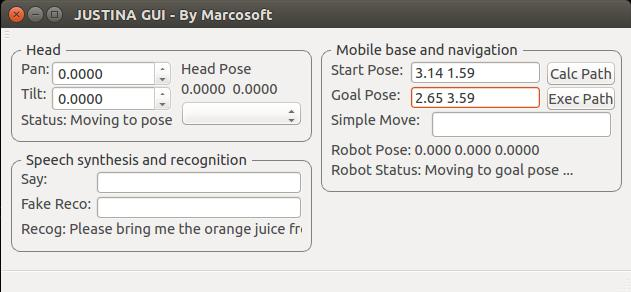
\includegraphics[width=0.65\textwidth]{Figures/gui.jpg}
\caption{Interfaz gráfica}
\label{fig:gui}
\end{figure}

Para correr todos los nodos necesarios (\texttt{map\_server, justina\_simple\_gui}) ejecute el comando
\begin{verbatim}
   roslaunch bring_up path_calculation.launch
\end{verbatim}

\subsection{Nodo que calcula y publica la ruta}
Crear un paquete de ROS con el nombre \texttt{path\_calculator} que tenga las siguientes características:
\begin{itemize}
\item Atender un servicio con el nombre \texttt{/navigation/a\_star}, de tipo \texttt{navig\_msgs/CalculatePath}, que calcule una ruta a partir de un mapa y posiciones inicial y final. 
\item La respuesta del servicio debe corresponder al éxito al calcular la trayectoria y la ruta resultante debe asignarse a la parte de respuesta del servicio.
\item En el \textit{callback} del servicio se deben ejecutar los algoritmos expuestos en la sección anterior: crecimiento de los obstáculos, cálculo de la ruta mediante A* y suavizado de la ruta (en ese orden).
\item Los obstáculos deben crecerse un número de celdas que equivalga a cuando menos 30 [cm].
\item Es tarea del alumno calcular los parámetros $\alpha$, $\beta$ y $\delta$ para el suavizado de la ruta.
\item El nodo debe publicar de manera periódica la última ruta calculada. El nombre del tópico debe ser \texttt{/navigation/a\_star\_path} de tipo \texttt{/nav\_msgs/Path}.
\item Todos los algoritmos deben estar contenidos en funciones o métodos bien definidos. No debe haber \textit{código espagueti}.
\end{itemize}

La figura \ref{fig:path} muestra un ejemplo del resultado esperado en \texttt{rviz}.
\begin{figure}
\centering
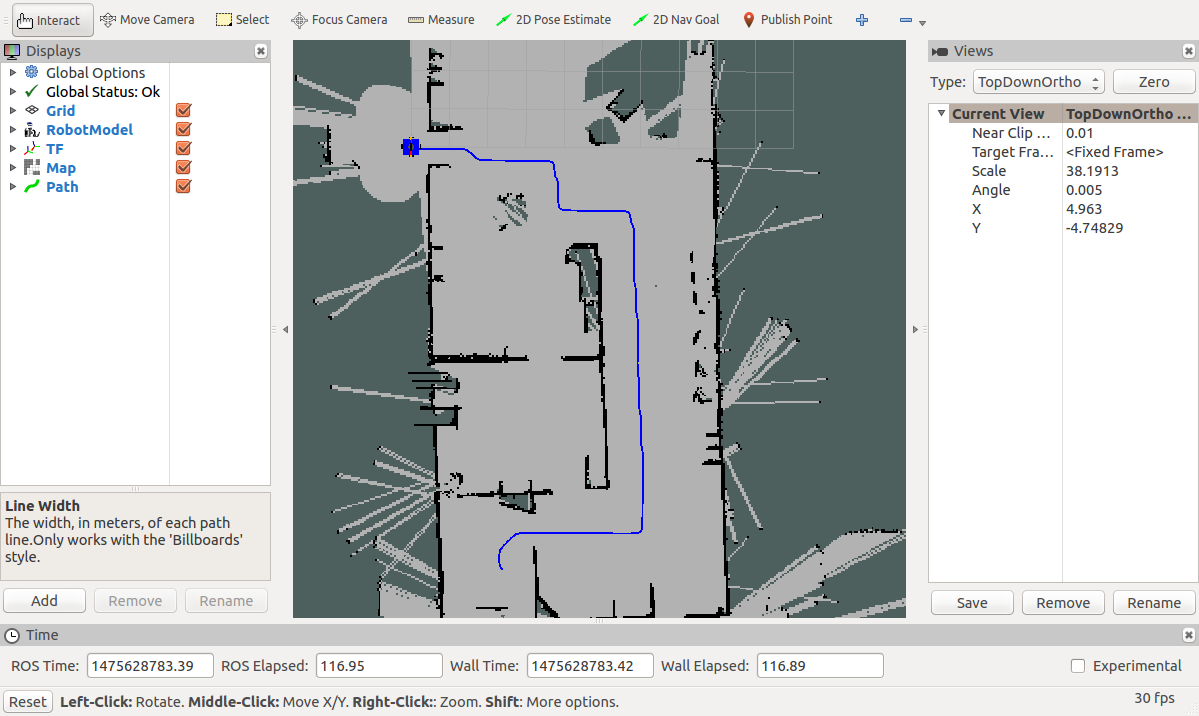
\includegraphics[width=0.9\textwidth]{Figures/Path.png}
\caption{Ejemplo de ruta calculada}
\label{fig:path}
\end{figure}

\section{Evaluación}
\begin{itemize}
\item El cálculo debe ser rápido (retardo no perceptible para un humano). 
\item El programa debe verificar que  inicio y meta NO estén en el espacio ocupado.
\item Se probabará con varios pares de posiciones iniciales y finales aleatorias.
\item Los parámetros de suavizado y el número de celdas que se aumenta a los obstáculos deben poderse cambiar fácilmente.
\item No es necesario que los valores anteriores se puedan cambiar en tiempo de ejecución. 
\item Las posiciones iniciales y finales sí se deben poder cambiar en tiempo de ejecución y se fijarán haciendo uso de la GUI.
\item El código debe estar ordenado.
\item \textbf{Importante: } Si el alumno no conoce su código, NO se contará la práctica.
\end{itemize}

\end{document}
%%% Local Variables:
%%% mode: latex
%%% TeX-master: t
%%% End:
